\chapter{Θεωρητικό υπόβαθρο}
Κατηγοριοποίηση Εικόνων με χρήση Συνελικτικών Νευρωνικών Δικτύων  

\section{Αναγνώριση Εικόνων}
\subsubsection{Πώς ένας υπολογιστής αναγνωρίζει εικόνες\;}
Η ταξινόμηση εικόνων περιγράφει ένα πρόβλημα στο οποίο σε ένα υπολογιστή δίνεται μία εικόνα και πρέπει να καταλάβει τι απεικονίζει (από ένα σύνολο πιθανών κατηγοριών)
Σήμερα, τα Συνελικτικά Νευρωνικά Δίκτυα \en{(CNNs)} αποτελούν  μια πολύ καλή  προσέγγιση αυτού το προβλήματος. Γενικά, τα νευρωνικά δίκτυα υποθέτουν πως υπάρχει κάποια συνάρτηση από την είσοδο (π.χ. εικόνες) σε μία έξοδο (π.χ. ένα σύνολο κατηγοριών εικόνων). Ενώ οι κλασσικοί αλγόριθμοι προσπαθούν να κωδικοποιήσουν  κάποια πληροφορία του πραγματικού κόσμου στη συνάρτηση τους, τα \en{CNN} μαθαίνουν την συνάρτηση δυναμικά  από ένα σύνολο ταξινομημένων εικόνων \en{(labelled images)}—αυτή η διαδικασία ονομάζετε εκπαίδευση. Μόλις καταλήξει σε μια σταθερή συνάρτηση (δηλαδή σε μια προσέγγιση αυτής), μπορεί να εφαρμόσει τη συνάρτηση σε εικόνες που δεν έχει ξαναδεί.

\subsubsection{Τι μπορεί να κάνει ένα νευρωνικό δίκτυο;}
Ένα νευρωνικό δίκτυο αποτελείται από πολλαπλά επίπεδα.  Κάθε επίπεδο λαμβάνει έναν πολυδιάστατο πίνακα αριθμών ως είσοδο και παράγει έναν άλλο πολυδιάστατο πίνακα αριθμών ως έξοδο (ο οποίος στη συνέχεια γίνεται η είσοδος του επόμενου επιπέδου). Κατά την ταξινόμηση εικόνων, η είσοδος του πρώτου επιπέδου είναι η εικόνα εισόδου  (π.χ.\( 32\times32\times3\) αριθμοί για εικόνες \(32\times32\) pixel με 3 κανάλια χρώματος), ενώ η έξοδος του τελευταίου επιπέδου αποτελείται  ένα σύνολο πιθανοτήτων των διαφόρων κατηγοριών (π.χ., \(1\times1\times10\) αριθμοί αν υπάρχουν \(10\) κατηγορίες).
 
Κάθε επίπεδο έχει ένα σύνολο από βάρη που σχετίζονται με αυτό — αυτά τα βάρη είναι που “μαθαίνει” το νευρωνικό όταν του δοθούν δεδομένα εκπαίδευσης. Ανάλογα με το επίπεδο, τα βάρη έχουν διαφορετικές ερμηνείες, αλλά δεν είναι αντικείμενο μελέτης του συγκεκριμένου \en{project}, φτάνει να γνωρίζουμε ότι κάθε επίπεδο λαμβάνει μία είσοδο, εκτελεί κάποια διεργασία σε αυτή, που εξαρτάται από τα βάρη και παράγει μια έξοδο. Αυτό το βήμα ονομάζεται εμπρόσθια διάδοση: παίρνουμε μία είσοδο και την προωθούμε στο δίκτυο, παράγοντας το επιθυμητό αποτέλεσμα ως έξοδο. Η εμπρόσθια διάδοση είναι το μόνο που χρειάζεται για την ταξινόμηση εικόνων σε ένα ήδη εκπαιδευμένο \en{CNN}.
 
Στην πράξη, ένα νευρωνικό δίκτυο αποτελεί μια πολύ απλή μηχανή αναγνώρισης προτύπων (με εξαιρετικά περιορισμένη χωρητικότητα), αλλά μπορεί να είναι αρκετά παράξενο αυτό που καταλήγει να αναγνωρίσει. Για παράδειγμα, κάποιος μπορεί να εκπαιδεύσει ένα νευρωνικό δίκτυο να αναγνωρίζει τη διαφορά μεταξύ “σκύλων” και “λύκων”, και να δουλέψει καλά κοιτώντας το χιόνι και το δάσος στο φόντο των φωτογραφιών με τους λύκους.

\section{Συνελικτικά Νευρωνικά Δίκτυα}
Συνελικτικά Νευρωνικά Δίκτυα \index{Νευρωνικά Δίκτυα}, \tl{Stanford} \cite{cs231n}.

Πηγή:
\begin{tabbing}
\src{https://cs231n.github.io/neural-networks-1/ }
\end{tabbing}

\subsection{Τι είναι τα Νευρωνικά Δίκτυα}

\subsubsection{Μοντελοποίηση ενός νευρώνα}

Οι νευρώνες είναι εμπνευσμένοι από τους βιολογικούς νευρώνες του ανθρώπινου νευρικού συστήματος. Παρακάτω φαίνεται μια απεικόνιση ενός βιολογικού νευρώνα και η μαθηματική μοντελοποίησή του. 

\begin{figure}[!ht] 
\centering
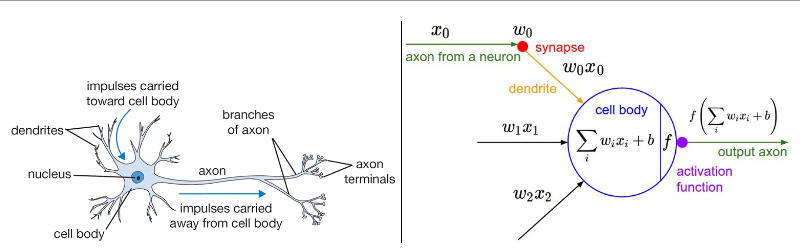
\includegraphics[width=\textwidth]{static/figures/cs231n_neuron.png} 
\caption{\en{A cartoon drawing of a biological neuron (left) and its mathematical model (right).}}
\label{neuron model}
\end{figure}

Κάθε νευρώνας λαμβάνει σήματα από τους δενδρίτες και παράγει ένα σήμα εξόδου στον άξονα. Στη συνέχεια ο άξονας διακλαδίζεται μέσω συνάψεων σε δενδρίτες άλλων νευρώνων. Στο υπολογιστικό μοντέλο τα σήματα ($x_0$) στον άξονα, αλληλοεπιδρούν πολλαπλασιαστικά μέσω των συνάψεων με τους δενδρίτες ($w_0 x_0$) . Οι συνάψεις θεωρούμε πως είναι τα εκπαιδεύσιμα  στοιχεία (βάρη $w$)  τα οποία ελέγχουν την επιρροή του ενός νευρώνα σε κάποιον άλλο. Στο κυρίως μέρος του νευρώνα, αθροίζονται τα σήματα από τους δενδρίτες. Εάν αυτό το άθροισμα ξεπερνά ένα συγκεκριμένο κατώφλι, ο νευρώνας ενεργοποιείται και στέλνει σήμα στον άξονα εξόδου. Στο μαθηματικό μοντέλο ο ακριβής χρόνος που παράγονται τα σήματα δεν έχει σημασία, η συχνότητα ενεργοποίησης του νευρώνα μας ενδιαφέρει. Ο τρόπος με τον οποίο το αναπαριστούμε  αυτό είναι με μια συνάρτηση ενεργοποίησης. Η πιο συνηθισμένη συνάρτηση είναι η σιγμοειδής, η οποία έχει σαν είσοδο μια πραγματική τιμή (την ισχύ του σήματος μετά το άθροισμα) και το περιορίζει στο διάστημα μεταξύ 0 και 1. Με άλλα λόγια, κάθε νευρώνας εκτελεί το εσωτερικό γινόμενο της εισόδου με τα βάρη προσθέτοντας και μία σταθερά (\en{bias}) και εφαρμόζει μία μη γραμμική συνάρτηση, σε αυτή την περίπτωση η σιγμοειδής  $\sigma(x)=1/(1+e-x)$ .

